\documentclass[thesis]{subfiles}

\begin{document}

\chapter{Protokół komunikacji}
\label{chapter:protokol}

Opracowany protokół komunikacji między serwerem i~klientem opiera się na~protokole~TCP. Bezpieczeństwo protokołu zapewnia wykorzystanie biblioteki OpenSSL. Oba te~elementy, tzn.~opracowany protokół aplikacji oraz~wykorzystana biblioteka OpenSSL, działają w~warstwie aplikacji modelu~TCP/IP, co~przedstawia tabela~\ref{fig:protocol-big-view}.

W~niniejszym rozdziale opisano wszystkie rodzaje pakietów przesyłanych między klientem i~serwerem oraz~sposób wykorzystania biblioteki OpenSSL w~projekcie.

\begin{table}
\renewcommand{\arraystretch}{1.5}
\begin{tabular}{l|l|l|l}
	   & Warstwy modelu OSI & Warstwy modelu TCP/IP~(DoD)       & Wykorzystane protokoły \\\hline\hline
	1. & Aplikacji          & \multirow{3}{*}{Aplikacji}        & \multirow{3}{*}{\parbox{3cm}{\textbf{Opracowany protokół + SSL}}} \\\cline{1-2}
	2. & Prezentacji        &                                   & \\\cline{1-2}
	3. & Sesji              &                                   & \\\hline
	4. & Transportowa       & Transportowa                      & TCP \\\hline
	5. & Sieciowa           & Internetu                         & IPv4 \\\hline
	6. & Łącza danych       & \multirow{2}{*}{Dostępu do sieci} & \multirow{2}{*}{Ethernet} \\\cline{1-2}
	7. & Fizyczna           &                                   &
\end{tabular}
\caption{Wykorzystane protokoły sieciowe i~ich umiejscowienie w~modelach OSI~i~TCP/IP~(DoD)}
\label{fig:protocol-big-view}
\end{table}

%------------------------------------------------------------------------------

\section{Rodzaje pakietów}

W~opracowanym protokole występuje kilka typów pakietów, które są~wysyłane między klientem i~serwerem. W~zależności od~etapu i~okoliczności komunikacji wykorzystywany jest różny typ pakietu. Pakiety są~łatwo rozróżnialne między sobą dzięki polu \texttt{TYPE} pakietu, określającym jego rodzaj. Pole \texttt{TYPE} jest częścią nagłówka pakietu. Nagłówek pakietu jest wspólny dla~wszystkich rodzajów pakietów. Rysunek~\ref{fig:packet-common} przedstawia schemat pamięci części wspólnej wszystkich pakietów, czyli nagłówek pakietu.

\begin{figure}
	\centering
	\begin{bytefield}{32}
		\bitheader{0,3,4,7,8,11,12,15,16,19,20,23,24,27,28,31}\\
		\begin{leftwordgroup}{Część wspólna\\wszystkich pakietów}
			\bitbox{4}{\texttt{VER}} & \bitbox{4}{\color{lightgray}\rule{\width}{\height}} & \bitbox{8}{TYPE} & \bitbox{8}{PKG\_MGR} & \bitbox{8}{\color{lightgray}\rule{\width}{\height}}
		\end{leftwordgroup}\\
		\begin{leftwordgroup}{Pola zależne\\od~typu pakietu}
			\wordbox[lrt]{2}{\vdots}\\
			\skippedwords\\
			\wordbox[lrb]{2}{\vdots}
		\end{leftwordgroup}\\
	\end{bytefield}
	\caption{Schemat wszystkich pakietów opracowanego protokołu}
	\label{fig:packet-common}
\end{figure}

Znaczenie poszczególnych pól w~nagłówku:\mynobreakpar
\begin{enumerate}
\item \texttt{VER} (\emph{Version}, 4~bity) --- Wersja protokołu. Jedyna akceptowalna wartość to~$1$. Pole to~zostało wprowadzone z~myślą o~ewentualnych przyszłych wersjach projektu, w~których mogłyby zajść duże zmiany w~układzie pól pakietów.
\item \texttt{TYPE} (8~bitów) --- Typ pakietu określający rolę jaką pakiet odgrywa w~komunikacji. Wszystkie typy pakietów zostały opisane w~dalszej części niniejszej pracy.
\item \texttt{PKG\_MGR} (\emph{Package manager}, 8~bitów) --- Rodzaj używanego przez klienta menadżera pakietów.
\end{enumerate}

W~tym rozdziale zostaną omówione rodzaje przesyłanych pakietów, wykorzystywanych w~opracowanym protokole m.in.~do~zarządzania oprogramowaniem klientów, obsługą sytuacji awaryjnych i~do~diagnostyki.

%---------------------------------------

\subsection{Żądanie aktualizacji}

Pakiet z~żądaniem aktualizacji oprogramowania jest przesyłany do~serwera przez klienta i~oznacza chęć dostosowania oprogramowania klienta do~wzorca serwera. Taki rodzaj pakietu jest symbolicznie oznaczany w~kodzie programu nazwą \texttt{FULL\_UPGRADE}. Nazwa ta, jak również nazwy innych pakietów przesyłanych w~ramach opracowanego protokołu, są~zdefiniowane jako typ wyliczeniowy~\texttt{enum~packet\_t} w~jednym z~plików nagłówkowych współdzielonych przez program serwera i~klienta. Typ pakietu jest przesyłany w~każdym pakiecie przesyłanym między klientem i~serwerem.

Serwer może mieć wiele wzorców oprogramowania dla~różnych klientów, dlatego klient przesyła do~serwera numer~wybranego zestawu konfiguracji. Numery konfiguracji odpowiadają różnym zapotrzebowaniom konfiguracji komputerów. Przykładowo, laboratorium komputerowe przeznaczone na~potrzebny nauki systemów CAD/CAM może mieć inny zestaw oprogramowania od~tego używanego w~salach w~bibliotece, co~może być odzwierciedlone w~przypisaniu innych numerów oprogramowania dla~komputerów w~tych salach.

\begin{figure}[h]
	\centering
	\begin{bytefield}{32}
		\bitheader{0,3,4,7,8,11,12,15,16,19,20,23,24,27,28,31}\\
		\begin{leftwordgroup}{Część wspólna\\wszystkich pakietów}
			\bitbox{4}{Version} & \bitbox{4}{\color{lightgray}\rule{\width}{\height}} & \bitbox{8}{Type} & \bitbox{8}{Distro} & \bitbox{8}{\color{lightgray}\rule{\width}{\height}}
		\end{leftwordgroup}\\
		\bitbox{16}{Config set} & \bitbox{16}{Not used}\\
		\wordbox{1}{Length}\\
		\begin{rightwordgroup}{Payload}
			\wordbox[lrt]{2}{$N$ data words}\\
			\skippedwords\\
			\wordbox[lrb]{2}{}
		\end{rightwordgroup}\\
		\begin{rightwordgroup}{Footer}
			\wordbox{1}{Checksum}
		\end{rightwordgroup}
	\end{bytefield}
	\caption{Pakiet~\texttt{FULL\_UPGRADE}}
	\label{fig:packet-full-upgrade}
\end{figure}

%------------------------------------------------------------------------------

\section{Bezpieczeństwo}
\label{sec:security}

Uwzględnienie bezpieczeństwa protokołu jest krytyczne dla projektu, ponieważ umożliwia on~serwerowi na zarządzanie konfiguracją wszystkich klientów. Zaniedbanie bezpieczeństwa protokołu lub~jego wadliwa implementacja, umożliwiłaby atakującemu system, na~przejęcie kontroli nad~wszystkimi klientami, np.~przez przesłanie klientom złośliwych aktualizacji oprogramowania lub~konfiguracji.

Umożliwienie przejęcia kontroli nad wszystkimi klientami byłoby prawdopodobnie najgorszym z~możliwych scenariuszy zarówno dla użytkowników jak i~administratora atakowanej sieci, jednak niedbała implementacja protokołu mogłaby umożliwiać również wiele innych rodzajów ataków, np. \emph{replay attack} i~\emph{man in the middle~(MITM)}. W~celu uniknięcia podatności protokołu na~wymienione i~inne, popularne rodzaje ataków, należy zagwarantować bezpieczeństwo protokołu co~najmniej pod względem:
\begin{enumerate}
\item uwierzytelnienia co~najmniej serwera,
\item poufności komunikacji,
\item integralności komunikacji.
\end{enumerate}
W~celu maksymalnego zaostrzenia rygorów bezpieczeństwa protokołu, do powyższych własności można dodać również inne, w~szczególności, własność \emph{\glslink{pfs}{Perfect Forward Secrecy~(PFS)}} (patrz rozdział~\ref{sec:pfs}).

W~kolejnych podrozdziałach zostaną opisane metody, które zostały wykorzystane do~zapewnienia poszczególnych elementów, składających się na~bezpieczeństwo protokołu. Wszystkie opisane dalej algorytmy i~metody kryptograficzne zostały wykorzystane przez niniejszy projekt przez wykorzystanie popularnej, otwartoźródłowej biblioteki kryptograficznej~\gls{openssl}, implementującej protokół kryptograficzny~\gls{ssl/tls}.

%---------------------------------------

\subsection{SSL/TLS}
\label{sec:ssl-tls}

Protokół \gls{ssl/tls} jest bardzo elastyczny pod względem doboru algorytmów i~metod kryptograficznych. Elastyczność objawia się nie tylko możliwością skonfigurowania konkretnych algorytmów, które posłużą do~zapewnienia uwierzytelnienia, poufności, integralności komunikacji i~ustalenia klucza sesji, ale również możliwością zdefiniowania za pomocą słów kluczowych, zbioru algorytmów spośród których serwer i~klient, podczas negocjacji w~ramach \emph{handshake'u} sesji \gls{ssl/tls}, wybierają jeden, najsilniejszy z~tych, które wspierają.

Przykładowo, jeśli celem jest dopuszczenie do~użytku wyłącznie zestawów metod kryptograficznych używających algorytmu \glslink{dh}{Diffiego-Hellmana} do~wymiany klucza, a~do szyfrowania szyfru blokowego~\gls{aes}, to filtr będzie miał postać napisu \texttt{DH+AES @STRENGTH}. Słowo kluczowe \texttt{@STRENGTH} służy do posortowania wynikowych zestawów metod kryptograficznych nierosnąco (a~nie ściśle malejąco) względem bezpieczeństwa.

Aby przekonać się jakie algorytmy zostaną zwrócone dla danego filtru, nie~trzeba korzystać z~\glslink{api}{API} biblioteki \gls{openssl}. Wystarczy nam do~tego konsola, co~prezentuje listing~\ref{openssl-console-filter}.\\

\begin{lstlisting}[numbers=none,language=bash,caption={Wynik filtrowania zestawów algorytmów w~konsoli za~pomocą \gls{openssl}},label=openssl-console-filter]
$ openssl ciphers -v 'DH+AES @STRENGTH'
AES256-GCM-SHA384   TLSv1.2 Kx=RSA  Au=RSA  Enc=AESGCM(256)  Mac=AEAD
AES256-SHA256       TLSv1.2 Kx=RSA  Au=RSA  Enc=AES(256)     Mac=SHA256
AES256-SHA          SSLv3 Kx=RSA    Au=RSA  Enc=AES(256)     Mac=SHA1
AES128-GCM-SHA256   TLSv1.2 Kx=RSA  Au=RSA  Enc=AESGCM(128)  Mac=AEAD
AES128-SHA256       TLSv1.2 Kx=RSA  Au=RSA  Enc=AES(128)     Mac=SHA256
AES128-SHA          SSLv3 Kx=RSA    Au=RSA  Enc=AES(128)     Mac=SHA1
\end{lstlisting}

Filtr złożony ze~słów kluczowych, wykorzystany w~implementacji projektu zarówno dla serwera, jak i~klienta, został przedstawiony na listingu~\ref{openssl-filter}. Filtr ten jest bardzo restrykcyjny, tak, aby zapewnić~\gls{pfs}. Wykrzyknik w filtrze pełni rolę operatora logicznego~\texttt{not}.\\

\begin{lstlisting}[numbers=none,caption={Filtr \gls{openssl} dla algorytmów użytych w~projekcie},label=openssl-filter]
kEECDH+ECDSA kEECDH kEDH +SHA !aNULL !eNULL !LOW !3DES !MD5 !EXP !DSS !PSK !SRP !kECDH !CAMELLIA !IDEA !RC4 !SEED @STRENGTH
\end{lstlisting}

Pełny opis słów kluczowych można znaleźć w~dokumentacji \gls{openssl} oraz w~darmowej, regularnie aktualizowanej elektronicznej książce\footnote{Jest ona częścią większej książki pt.~,,Bulletproof SSL and TLS"~(ISBN:~978-1907117046). Projekt \gls{openssl} ma~raczej opinię słabo udokumentowanego, dlatego te~książki mają spore znaczenie praktyczne.} pt.~,,OpenSSL Cookbook" autorstwa Ivana Ristić'a, polecanej na~oficjalnej stronie internetowej projektu~\gls{openssl}~\cite{openssl-cookbook-suites}.

%---------------------------------------

\subsection{Uwierzytelnienie}

Uwierzytelnienie serwera przez klienta jest krytyczne dla~bezpieczeństwa protokołu. Gdyby nie ono, to~atakujący mógłby podawać się za~serwer i~przesłać klientowi dowolną konfigurację i~oprogramowanie. Gdyby komunikacja była szyfrowana, ale nieuwierzytelniona, to atakujący mógłby również podjąć próby ataku \emph{replay attack}. W~celu uniknięcia tego problemu wykorzystano certyfikat X.509 dla~serwera~\cite{wiki:x509}.

Wygenerowanie takiego certyfikatu wymaga podpisania przez centrum certyfikacji~(\gls{ca})~\cite{wiki:ca}. Ze~względu na~brak potrzeby posiadania w~trakcie implementacji certyfikatu podpisanego przez uznane \gls{ca}, a~także ze względu na~względnie duże koszty finansowe i~czasowe z~tym związane, w czasie implementacji wykorzystano certyfikat podpisany przez siebie~(ang.~\emph{self-signed certificate}). Konfiguracja klienta pozwala w~trybie \texttt{debug} zaufać takiemu certyfikatowi. Oczywiście, w~przypadku wdrożenia projektu, należałoby postarać się o~certyfikat podpisany przez uznany~\gls{ca}.

Wygenerowanie i~podpisanie certyfikatu zostało wykonane z~użyciem \gls{openssl}. Listing~\ref{openssl-gencert} przedstawia jak wygenerować klucze publiczny i~prywatny \gls{rsa} o~długości 4096~bitów, a~następnie, jak wykorzystać klucz prywatny do~wygenerowania żądania podpisania certyfikatu (ang.~\emph{Certificate signing request}) i~na jego podstawie podpisać certyfikat~X.509~\cite{openssl-cookbook,wiki:csr}.

\begin{lstlisting}[numbers=none,caption={Wygenerowanie i~podpisanie certyfikatu X.509},label=openssl-gencert]
$ openssl genrsa -aes256 -out rsa_aes256_4096.key 4096
$ openssl req -new -key rsa_aes256_4096.key -out request.csr
$ openssl req -new -config request.cnf -key fd.key -out request.csr
$ openssl x509 -req -days 365 -in request.csr -signkey rsa_aes256_4096.key -out certificate.pem
\end{lstlisting}

Przykładowa zawartość pliku \path{request.cnf}, który służy do~konfiguracji żądania podpisania certyfikatu przedstawia listing~\ref{openssl-request-config}.

\begin{lstlisting}[numbers=none,caption={Plik z~konfiguracją certyfikatu X.509},label=openssl-request-config]
[req]
default_bits       = 4096
default_keyfile    = rsa_aes256_4096.key
prompt             = no
distinguished_name = dn
req_extensions     = ext
input_password     = minipw

[dn]
CN                 = Patryk
OU                 = MiNI
emailAddress       = patryk.beza@gmail.com
O                  = PW
L                  = Warsaw
ST                 = Masovian
C                  = PL

[ext]
subjectAltName     = DNS:www.mini.pw.edu.pl,DNS:*.mini.pw.edu.pl
\end{lstlisting}

Aby sprawdzić czy~certyfikat jest przez nas zaufany, wystarczy wydać komendę:
\begin{lstlisting}[numbers=none]
$ openssl verify -verbose certificate.pem
\end{lstlisting}

%---------------------------------------

\subsection{Poufność}

Poufność komunikacji nie jest tak krytyczna jak uwierzytelnienie serwera, jednak jest również istotna, ponieważ atakujący podsłuchujący komunikację między serwerem i~klientami, mógłby się~wiele dowiedzieć o~wersjach i~konfiguracji oprogramowania klientów. Dzięki zdobytej wiedzy, atakujący mógłby przeanalizować np.~czy oprogramowanie klientów jest przestarzałe i~podatne na~ataki, czy konfiguracja oprogramowania pozwala na~wykorzystanie luk bezpieczeństwa.

Komunikacja między serwerem i~klientem jest szyfrowana symetrycznym, blokowym szyfrem \gls{aes} z~kluczem 256-bitowym~(preferowane podczas negocjacji) lub~128-bitowym. Dla~obu długości klucza możliwe jest działanie w~trybie~GCM\footnote{\emph{Galois/Counter Mode}.}~(preferowane) lub~domyślnym.

%---------------------------------------

\subsection{Integralność}

Integralność komunikacji jest konieczna, aby zapobiec atakom typu \emph{man in the middle}, polegającym na~modyfikacji komunikacji między serwerem i~klientem, niezależnie od~tego czy jest ona~szyfrowana czy nie.

Algorytm używany do~sprawdzania integralności wiadomości jest negocjowany tak jak algorytmy używane do~zapewnienia uwierzytelnienia, szyfrowania i~ustalenia wspólnego klucza dla symetrycznego algorytmu szyfrującego komunikację (patrz rozdział~\ref{sec:ssl-tls}). Możliwe algorytmy to: \emph{AEAD}\footnote{Ściśle rzecz biorąc tryb AEAD~(ang.~\emph{Authenticated Encryption with Associated Data}) jest klasą wiązania bloków zaszyfrowanych w~blokowym algorytmie szyfrującym (ang.~\emph{Block cipher mode of operation}. \gls{aes} pracujący w trybie GCM należy do~tej klasy, dzięki czemu integralność jest zapewniana ,,przy okazji" szyfrowania komunikacji.}, \emph{SHA384}, \emph{SHA256} i~\emph{SHA1}.

%---------------------------------------

\subsection{Perfect Forward Secrecy}
\label{sec:pfs}

Własność \emph{\glslink{pfs}{Perfect Forward Secrecy}~(PFS)} umożliwia zachowanie poufności komunikacji nawet jeśli atakujący zapisał całą zaszyfrowaną komunikację między serwerem i~klientem, a~po~jakimś czasie uzyskał klucze prywatne obu stron komunikacji. Własność ta~wiąże się ze sposobem ustalenia sesyjnego klucza dla~symetrycznego szyfru zapewniającego poufność komunikacji (takiego jak np.~\gls{aes}).

W~uproszczeniu problem polega na tym, że~w~przypadku wykorzystania~\gls{rsa} do~ustalenia klucza sesyjnego dla~symetrycznego algorytmu szyfrującego, strona~A komunikacji, używa klucza publicznego strony~B do~zaszyfrowania losowego klucza sesyjnego\footnote{W~rzeczywistości \emph{Pre-Master Key}, z~którego dopiero jest wyliczany ostateczny klucz sesyjny.}~i wysyła go~do~B. Po~skompromitowaniu klucza prywatnego strony~B, atakujący może odczytać całą komunikację między stronami A~i~B, deszyfrując najpierw klucz sesyjny, a~następnie całą komunikację między serwerem i~klientem.

\gls{pfs} radzi sobie z~tym problemem rezygnując z~przesyłania zaszyfrowanego klucza sesyjnego, wprowadzając zamiast tego efemeryczny algorytm \glslink{dh}{Diffiego-Hellmana} w~postaci klasycznej~(\glslink{dh}{EDH})~i krzywoeliptycznej~(ECDHE)~\cite{mimuw-ssl-w04,openssl-cookbook-suites}. Efemeryczny algorytm \glslink{dh}{Diffiego-Hellmana} różni się od~nieefemerycznego tym, że~w~efemerycznej wersji algorytmu parametry algorytmu nie~są stałe, tzn. np.~nie są zapisane w~certyfikacie. Wersja krzywoliniowa co do~pomysłu nie różni się istotnie od~wersji klasycznej, tylko działa na krzywych eliptycznych. Wersja krzywoeliptyczna charakteryzuje się~lepszą wydajnością na~większości procesorów ze~względu na~fakt, że~do zapewnienia takiego samego poziomu bezpieczeństwa jakie gwarantuje~\gls{rsa} z~kluczem o~długości 3072~bitów, potrzeba krzywoeliptycznego odpowiednika o~długości 256~bitów.

Poniżej został przedstawiony schemat przebiegu klasycznego algorytmu \glslink{dh}{Diffiego-Hellmana}.

\begin{enumerate}
\item A i~B uzgadniają skończoną, cykliczną grupę~$G$ rzędu~$p$, gdzie $p$ jest liczbą pierwszą i~generator $g$ tej grupy. Atakujący może znać~$g$ oraz~$p$.
\item A wybiera tajną liczbę całkowitą $1 \leq a < n$ i~wysyła do~B liczbę $A=g^a \pmod{p}$.
\item B wybiera tajną liczbę całkowitą $1 \leq b < n$ i~wysyła do~A liczbę $B=g^b \pmod{p}$.
\item A oblicza $s=B^a \pmod{p}$.
\item B oblicza $s=A^b \pmod{p}$.
\item A i~B współdzielą tajną liczbę~$s$.
\end{enumerate}

Podsłuchujący atakujący, aby~poznać liczbę $s$, musiałby rozwiązać tzw.~problem Diffiego-Hellmana, który jest problemem równie trudnym w~sensie teorii złożoności, jak problem algorytmu dyskretnego. Liczby $a$ i~$b$ są~przed wysłaniem podpisywane kluczem prywatnym w celu uniknięcia ataku~\emph{man in the middle}.

Ilustracja~\ref{fig:dh} obrazowo przedstawia w~jaki sposób działa algorytm \glslink{dh}{Diffiego-Hellmana}.

\begin{figure}[hb]
	\centering
	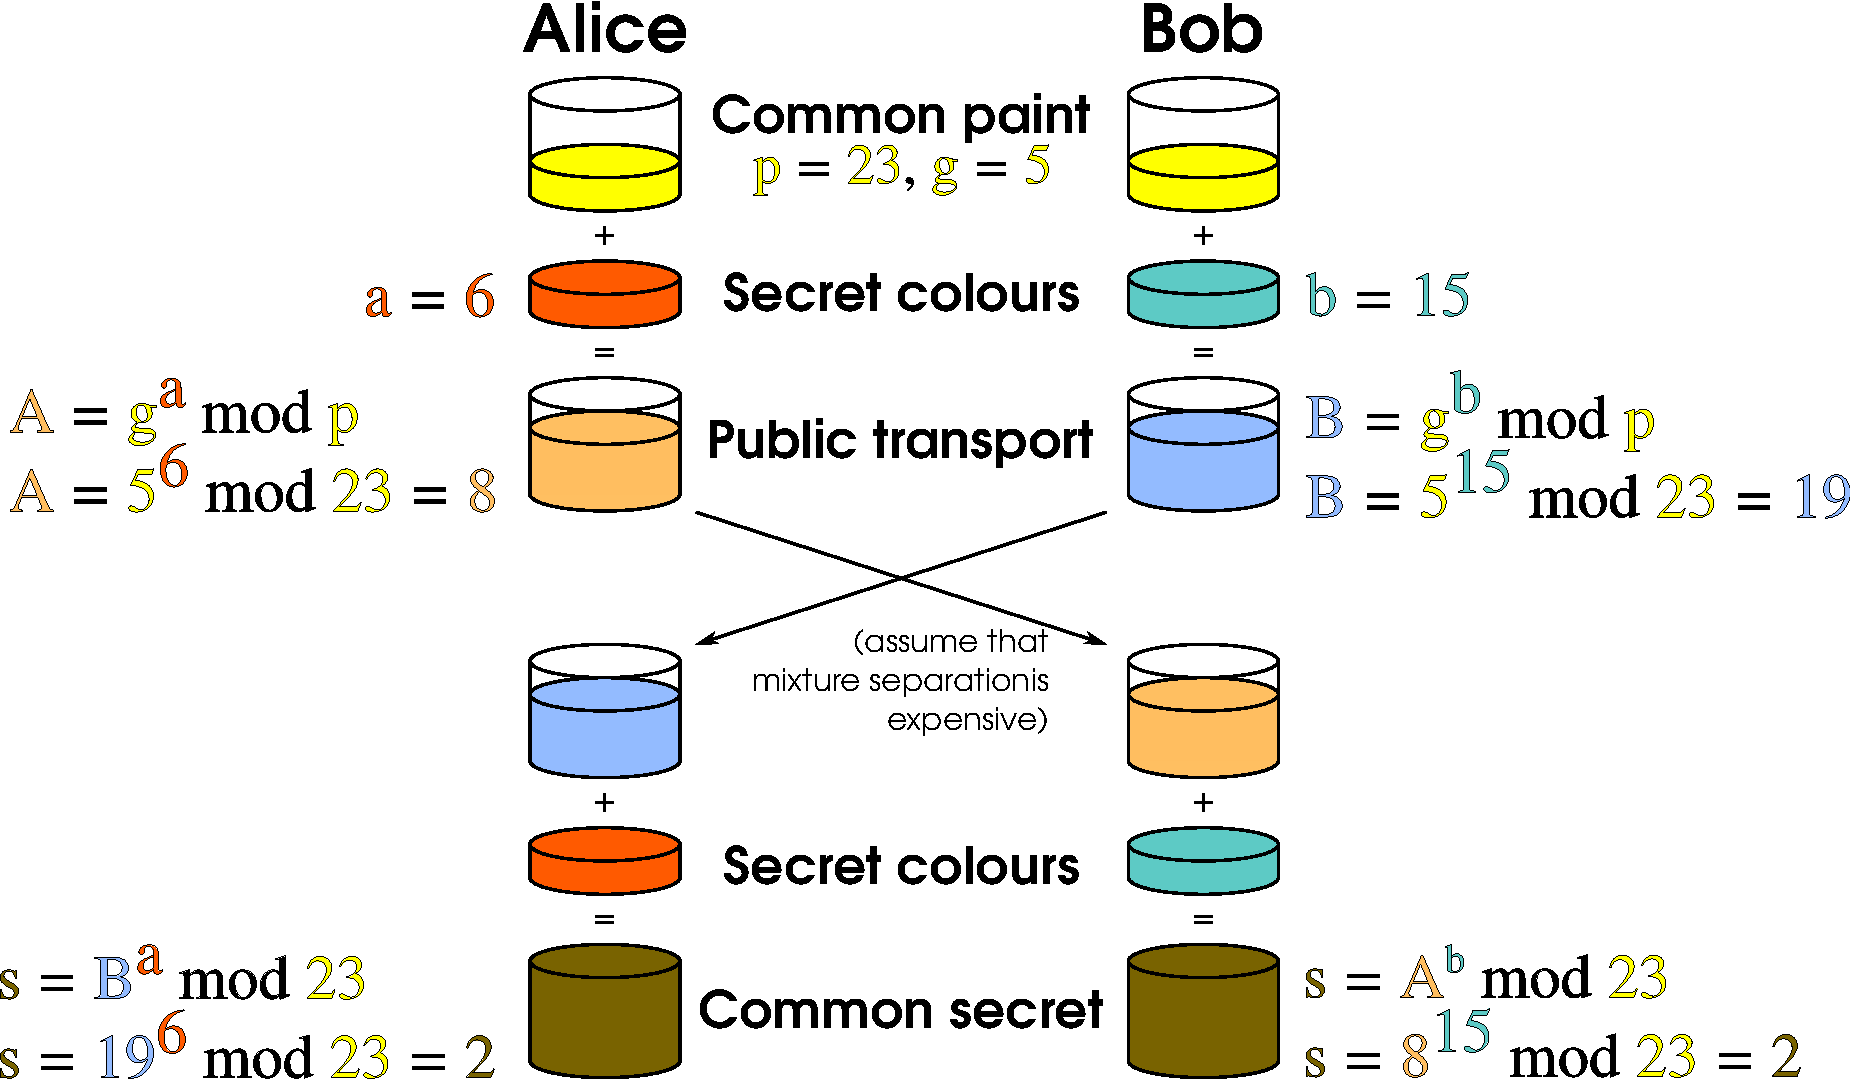
\includegraphics[width=\textwidth]{img/Diffie-Hellman_Key_Exchange_desc}
	\caption{Zobrazowanie działania algorytmu Diffiego-Hellmana (źródło: Wikipedia)}
	\label{fig:dh}
\end{figure}

%---------------------------------------

\subsection{Zestawy kryptograficzne}

W~praktyce, podczas testów, w~czasie których nawiązywano połączenie \gls{ssl/tls} pomiędzy klientem i~serwerem uruchamianym na~systemie z~zainstalowanym \gls{openssl} w~wersji \texttt{1.0.2h}, strony połączenia zawsze negocjowały zestaw algorytmów \texttt{ECDHE-RSA-AES256-GCM-SHA384}, który oznacza użycie najnowszego dostępnej wersji protokołu~\glslink{ssl/tls}{TLS}, tj.~protokołu~TLSv1.2, zapewniającego:
\begin{enumerate}
\item Poufność przez wykorzystanie \gls{aes} pracującym w trybie GCM z~kluczem o~długości 256~bitów,
\item Ustalenie klucza sesyjnego dla~\gls{aes} przez~wykorzystanie efemerycznej wersji algorytmu \glslink{dh}{Diffiego-Hellmana} w~wersji dla~krzywych eliptycznych~(ECDH),
\item Uwierzytelnienie przez wykorzystanie podpisu cyfrowego z~wykorzystaniem~\gls{rsa},
\item Integralność gwarantowaną przez działanie \gls{aes} w~trybie~GCM. SHA384~w~nazwie wynegocjonowanego zestawu oznacza uczycie funkcji haszującej SHA384 podczas fazy \emph{handshake} i~do rozszerzenia dzielonego sekretu uzyskanego podczas ustalenia klucza~sesyjnego do~klucza symetrycznego dla~\gls{aes}~\cite{stack:openssl-sha-gcm}.
\end{enumerate}

\end{document}
